\begin{figure}[bl]
  \vspace{-1.0em}
  \centering
  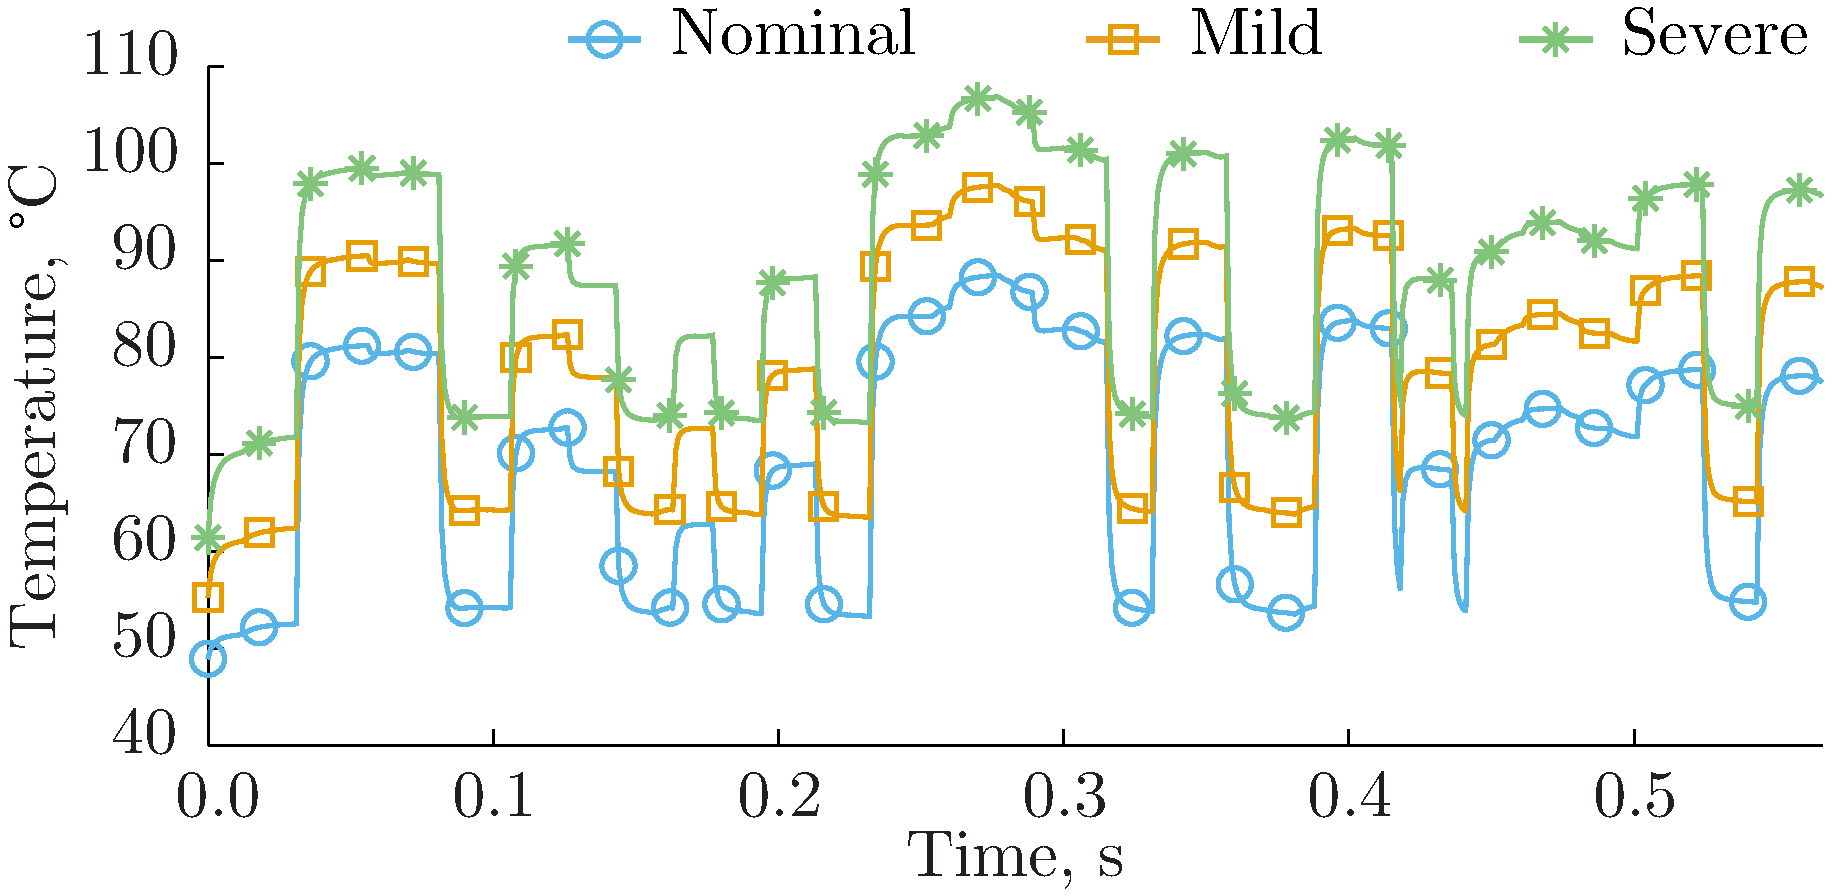
\includegraphics[width=1.0\linewidth]{include/assets/motivation-temperature.pdf}
  \vspace{-1.5em}
  \caption{Temperature fluctuation due to process variation.}
  \flabel{motivation-temperature}
\end{figure}

Process variation constitutes one of the major concerns of electronic system designs \cite{chandrakasan2001, srivastava2010}.
A crucial implication of process variation is that it renders the key parameters of a technological process, \eg, the effective channel length, gate oxide thickness, and threshold voltage, as random quantities.
Therefore, the same workload applied to two ``identical'' dies can lead to two different power and, thus, temperature profiles since the dissipation of power and heat essentially depends on the aforementioned stochastic parameters.
Consequently, process variation leads to performance degradation in the best case and to severe faults or burnt silicon in the worst scenario.
Under these circumstances, uncertainty quantification \cite{xiu2010, maitre2010} has evolved into an indispensable asset of electronic system design workflows providing them with guaranties on the efficiency and robustness of products.

In order to illustrate the above concern, consider a quad-core architecture exposed to the uncertainty of the parameters that affect the leakage current.
Assume first that these parameters have nominal values.
We can then simulate the system under a certain workload and observe the corresponding temperature profile.\footnote{The experimental setup will be detailed in \sref{illustrative-example} and \sref{experimental-results}.}
The result, labeled as ``Nominal'', is depicted in \fref{motivation-temperature} where, for clarity, only one curve, corresponding to one processor, is presented (the bottom blue line). It can be seen that the temperature is always below $90^{\circ}$C.
Now let us assume a mild deviation of the parameters from the nominal values and run the simulation once again. The result is the ``Mild'' curve in \fref{motivation-temperature} (the middle orange line); the maximal temperature is approaching $100^{\circ}$C.
Finally, we repeat the experiment considering a severe deviation of the parameters and observe the curve labeled as ``Severe'' in \fref{motivation-temperature} (the top green line); the maximal temperature is almost $110^{\circ}$C.
Imagine that the designer, when tuning the solution constrained by a maximal temperature of $90^\circ$C, was guided exclusively by the nominal parameters.
In this case, even with mild deviations, the circuits might be burnt, and the amount of burnt circuits depends on the probability distribution of temperature.
Such uncertainties have to be addressed in order to pursue efficiency and fail-safeness.
Nevertheless, the majority of the literature related to power-temperature analysis of multiprocessor systems ignores this important aspect, \eg, \cite{rao2009, rai2011, thiele2011, ukhov2012}.

The remainder of the paper is organized as follows.
\sref{prior-work} provides an overview of the prior work.
In \sref{present-work}, we summarize the contribution of the present paper.
The objective of our study is formulated in \sref{problem-formulation}.
The proposed framework is presented in \sref{proposed-framework}.
A particular application of our approach is discussed in \sref{illustrative-example}, and the corresponding results are compared with MC simulations in \sref{experimental-results}.
\sref{conclusion} concludes the paper.
The work contains a set of supplementary materials with discussions on certain aspects of our framework.
